\PassOptionsToPackage{svgnames}{xcolor}
\documentclass[mathserif]{beamer}

\let\emph\textbf

\usepackage[english]{babel}
\usepackage[utf8]{inputenc}
\usepackage{lmodern}
\usepackage[T1]{fontenc}
\usepackage{datetime}
\usepackage{xifthen}

\usepackage{amsmath,amssymb}
\usepackage{mathtools}
\usepackage{geometry}
\usepackage{hyperref}
\usepackage{microtype}
\usepackage{verbatim}
\usepackage{rotating}
\usepackage{array}
\usepackage[ruled,linesnumbered]{algorithm2e}

\usepackage{xspace}
\newcommand{\ie}{i.e.\@\xspace}
\newcommand{\eg}{e.g.\@\xspace}
\newcommand{\etal}{et al.\@\xspace}

\newcommand{\N}{\mathbb{N}}
\newcommand{\Z}{\mathbb{Z}}
\newcommand{\Q}{\mathbb{Q}}
\newcommand{\GF}[2][2]{\mathbb{F}_{#1^{#2}}}
\newcommand{\T}{\mathcal{T}}
\newcommand{\set}[1]{\left\{ #1 \right\}}
\newcommand{\card}[1]{\left| #1 \right|}
\DeclareMathOperator{\lcm}{lcm}
\DeclareMathOperator{\Tr}{Tr}
\makeatletter
\newcommand{\tr}[3][1]{\ifthenelse{\isempty{#3}}%
  {\Tr_{#1}^{#2}}%
  {\Tr_{#1}^{#2}\left(#3\right)}}
\newcommand{\addch}[1]{\ifthenelse{\isempty{#1}}%
  {(-1)}%
  {(-1)^{#1}}}
\newcommand{\mulch}[2][m_1]{\ifthenelse{\isempty{#2}}%
  {\psi_{#1}}%
  {\psi_{#1} \left( #2 \right)}}
\makeatother
\newcommand{\WT}[1]{\widehat{#1}}
\newcommand{\Snu}[1][\nu]{S_{#1}(a, b, \omega)}
\newcommand{\mystery}{h_{a, b}(\omega)}

\hypersetup{pdftitle={A conjecture about Gauss sums and bentness of binomial Boolean functions},%
  pdfauthor={Jean-Pierre Flori},%
  pdfsubject={Mathematics and Cryptography},%
  pdfcreator={Jean-Pierre Flori},%
  pdfproducer={Jean-Pierre Flori},%
  pdfkeywords={mathematics} {cryptography} {Boolean functions} {bent functions} {Walsh spectrum} {Kloosterman sums},
}


\usepackage{tikz}
\usetikzlibrary{arrows, positioning, calc, matrix, fit, snakes}
\usepackage{pgfplots}

\usetheme{Madrid}
\usefonttheme{structurebold}
%\setbeamertemplate{footline}[frame number]{}
\beamertemplatenavigationsymbolsempty

\newtheorem{proposition}{Proposition}
\newtheorem{conjecture}{Conjecture}

\newcommand{\blue}[1]{\textcolor{blue}{#1}}
\newcommand{\red}[1]{\textcolor{red}{#1}}
\newcommand{\cone}[1]{\textcolor{blue}{#1}}
\newcommand{\ctwo}[1]{\textcolor{red}{#1}}
\newcommand{\cthree}[1]{\textcolor{Green}{#1}}
\newcommand{\cthreebis}[1]{\textcolor{Teal}{#1}}
\newcommand{\cfour}[1]{\textcolor{orange}{#1}}
\newcommand{\cfive}[1]{\textcolor{violet}{#1}}

\title[Gauss sums and binomial functions]{A conjecture about Gauss sums and bentness of binomial Boolean functions}

\author[JPF]{\blue{Jean}-Pierre \red{Flori}}

\institute[ANSSI]{\blue{Agence nationale} de la sécurité \red{des systèmes d'information}}

\date[16/07/14]{\blue{July} 14, \red{2016}\\\blue{WAIFI 2016,} Ghent, \red{Belgium}}

\begin{document}

\begin{frame}
  \titlepage
\end{frame}

\begin{frame}
  \begin{definition}
    A Boolean function $f: \GF{n} \rightarrow \GF{}$ is said to be \emph{bent}
    if its Fourier/Walsh transform $\WT{f}(\omega) = \sum_{x \in \GF{n}} (-1)^{f(x) + \tr{n}{\omega x}}$ is always $\pm 2^{n/2}$.
  \end{definition}

  \begin{itemize}
  \item Bent functions are as non-linear as possible.
  \item Applications in cryptography, coding theory.
  \end{itemize}

  \begin{itemize}
  \item No known classification.
  \item Above definition not practical.
  \end{itemize}

  \vspace{1em}

  \begin{alertblock}{Problem}
    Devise infinite families of functions with efficient characterizations for bentness.
  \end{alertblock}
\end{frame}

\begin{frame}
  \begin{example}[Dillon's monomial]
    There exist infinite families of bent functions of the form $f_a(x) = \tr{n}{a x^{2^{m}-1}}$ with $n = 2m$ and $a \in \GF{m}^*$.
  \end{example}

  \begin{definition}[Kloosterman sum]
    The \emph{Kloosterman sum} associated with $a$ is
    \[
    K_m(a) = \sum_{x \in \GF{m}}\addch{\tr{m}{ax + x^{-1}}} \enspace .
    \]
  \end{definition}

  \begin{itemize}
  \item Kloosterman sums are related to number of points on elliptic curves.
  \item They can be computed (very) efficiently.
  \item And characterize bentness of $f_a$ (and more)!
  \end{itemize}

  \begin{theorem}[Dillon's monomial]
    $f_a(x)$ is bent iff $K_m(a) = 0$.
  \end{theorem}
\end{frame}

\begin{frame}
  \begin{theorem}[Mesnager's binomial]
    For $n = 2 m$ with $m$ odd, $a \in \GF{m}^*$, and $b \in \GF[4]{}^*$, the Boolean function $f_{a,b}(x) = \tr{n}{a x^{2^{m}-1}} + \tr{2}{b x^{(2^n - 1)/3}}$ is bent iff $K_m(a) = 4$.
  \end{theorem}

  The proof gives an explicit formula for the Walsh transform and
  relies on three main ingredients:
  \begin{itemize}
  \item the \emph{polar decomposition} of finite fields,
  \item properties of \emph{Dickson polynomials},
  \item values of \emph{cubic sums}.
  \end{itemize}
  But it does not apply when $m = n/2$ is even.

  \vspace{1em}

  \begin{alertblock}{This work}
    Partially compute the Walsh transform when $m$ is even.
  \end{alertblock}
\end{frame}

\begin{frame}
  In general the condition remains \emph{necessary}.
  \begin{proposition}[Mesnager]
    For any $n = 2 m$, if $f_{a,b}(x)$ is bent, then $K_m(a) = 4$.
  \end{proposition}

  \vspace{2em}

  And for small parameters it remains \emph{sufficient}.
  \begin{proposition}[Flori, Mesnager, Cohen]
    For $n = 2 m$ up to $32$, if $K_m(a) = 4$, then $f_{a,b}(x)$ is bent.
  \end{proposition}

  \vspace{2em}

  \begin{itemize}
  \item Can we prove it always is sufficient? \emph{Not yet}.
  \item But some progress was made, especially when \emph{$n = 4m$ with $m$ odd}.
  \end{itemize}
\end{frame}

\begin{frame}
  \begin{definition}[Polar decomposition]
    Let $n = 2 m$, then $\GF{n}^* \simeq U \times \GF{m}^*$ where $U \subset \GF{n}^*$ is the subgroup of $(2^m+1)$-th roots of unity (and $\GF{m}^*$ that of $(2^m-1)$-th roots of unity).
  \end{definition}
  \begin{itemize}
  \item This decomposition can be \textbf{iterated} as long as $n = 2^\nu m$ is even.
  \item The value of $f_{a,b}(x) = \tr{n}{a x^{2^{m}-1}} + \tr{2}{b x^{(2^{n}-1)/3}}$ only depends on the \textbf{polar part} in $U$.
  \end{itemize}

  \begin{lemma}
    Let $n = 2^\nu m$ with $m$ odd, then
    \[
    \WT{f}(\omega) = 1 - \cone{\sum_{u \in U} \addch{f_{a,b}(u)}} + 2^{m} \ctwo{\sum_{u \in U, \tr[m]{n}{\omega u} = 0} \addch{f_{a,b}(u)}} \enspace .
    \]
  \end{lemma}

  \begin{itemize}
  \item When \cone{$\nu = 1$}, evaluating the \cone{first sum} is the hard part.
  \item When \ctwo{$\nu > 1$}, evaluating the \ctwo{second sum} is the hard part.
  \end{itemize}
\end{frame}

\begin{frame}
  \textbf{From now on, $\nu = 2$, $n = 4 m$ with $m$ odd, and $m_i = n / 2^i$.}

  \begin{itemize}
  \item Polar decomposition: $\GF{n}^* \simeq U_1 \times U_2 \times \GF{m_2}^* \simeq U \times \GF{m_2}^*$.
  \item $f_{a,b}$ decomposes \emph{additively}:
    \begin{align*}
    f_{a,b}(x) & = \tr{n}{a u_1^{2^{m_1}-1}} + \tr{2}{b u_2^{(2^{m_0}-1)/3}} \\
      & = f_{a}(u_1) + g_{b}(u_2) \enspace .
    \end{align*}
  \item And the \cone{first sum} decomposes \emph{multiplicatively}:
    \[
    \cone{\Sigma_1} = \sum_{u_1 \in U_1} \addch{f_{a}(u_1)} \sum_{u_2 \in U_2} \addch{g_{b}(u_2)} \enspace .
    \]
  \end{itemize}

  \begin{lemma}
    \[
    \cone{\Sigma_1} = - \frac{2^{m_2} + 1}{3} \left( 1 - K_{m_1}(a) \right) \enspace .
    \]
  \end{lemma}
\end{frame}

\begin{frame}
  The \ctwo{second sum}
  \[
  \ctwo{\Sigma_2} = \sum_{u \in U, \tr[m_2]{m_0}{\omega u} = 0} \addch{f_{a}(u_1)}\addch{g_{b}(u_2)}
  \]
  is conditioned by a trace down to the odd degree extension:
  \begin{itemize}
  \item either $\tr[m_1]{m_0}{\omega u} = 0$, and then $u_1 = \omega_1^{-1}$,
  \item or $\tr[m_1]{m_0}{\omega u} \neq 0$, and then $u_1 \neq \omega_1^{-1}$ and $u_2$ is the polar part of $\left( \omega_2 \tr[m_1]{m_0}{\omega_1 uu_1} \right)^{-1}$.
  \end{itemize}

  \begin{lemma}
    \begin{align*}
    \ctwo{\Sigma_2} = & - \frac{2^{m_2} + 1}{3} \addch{f_{a}(\omega_1^{-1})} \\
    & \qquad + \cthree{\sum_{u_1 \neq \omega_1^{-1}} \addch{f_{a}(u_1)} \addch{g_{b}\left(\left( \omega_2 \tr[m_1]{m_0}{\omega_1 u_1} \right)^{-1}\right)}} \enspace .
    \end{align*}
  \end{lemma}
\end{frame}

\begin{frame}
  Evaluating the \cthree{third sum}
  \[
  \cthree{\Sigma_3} = \sum_{u_1 \neq \omega_1^{-1}} \addch{f_{a}(u_1)} \addch{g_{b}\left(\left( \omega_2 \tr[m_1]{m_0}{u_1 \omega_1} \right)^{-1}\right)}
  \]
  is equivalent to evaluating
  \[
  \cthreebis{\Sigma_3^\gamma} = \sum_{\substack{u_1 \neq 1,\\ \left( u_1 + u_1^{-1} \right)^{(2^{m_1}-1)/3} = \gamma}} \addch{\tr{m_0}{a \omega_1^2 u_1}} \enspace .
  \]
  (The sum \cthreebis{$\Sigma_3^\gamma$} is slightly easier to compute than
  the Walsh transform in practice.)

  \vspace{2em}

  Unfortunately, we cannot go much further, \emph{unless $\omega_1 = 1$}.
\end{frame}

\begin{frame}
  \textbf{From now on, $\omega_1 = 1$}
  \[
  \cthreebis{\Sigma_3^\gamma} = \sum_{\substack{u_1 \neq 1,\\ \left( u_1 + u_1^{-1} \right)^{(2^{m_1}-1)/3} = \gamma}} \addch{\tr{m_1}{a (u_1 + u_1^{-1})}} \enspace .
  \]

  \begin{proposition}[Hilbert's Theorem 90]
    The map $x \mapsto x + x^{-1}$ is $2$-to-$1$ from $U_1 \backslash \{1\}$ to $T_1 = \left\{x \in \GF{m_1}^* | \tr{m_1}{1/x} = 1\right\}$ and from $\GF{m_1}^* \backslash \{1\}$ to $T_0 = \left\{x \in \GF{m_1}^* | \tr{m_1}{1/x} = 0\right\}$.
  \end{proposition}

  \vspace{1em}

  The \cthreebis{third sum} is now just a sum over (part of) $\GF{m_1}$:
  \[
  \cthreebis{\Sigma_3^\gamma} = 2 \sum_{\substack{ t \in T_1,\\ t^{(2^{m_1}-1)/3} = \gamma}} \addch{\tr{m_1}{a t}} \enspace .
  \]
\end{frame}

\begin{frame}
  The usual trick to evaluate such sums on $T_1$ is to artificially add $\tr{m_1}{1/t}$ and to sum over all of $\GF{m_1}$:
  \[
  \cthreebis{\Sigma_3^\gamma} = \sum_{\substack{ t \in \GF{m_1},\\ t^{(2^{m_1}-1)/3} = \gamma}} \addch{\tr{m_1}{a t}} - \sum_{\substack{ t \in \GF{m_1},\\ t^{(2^{m_1}-1)/3} = \gamma}} \addch{\tr{m_1}{a t + t^{-1}}} \enspace .
  \]

  \vspace{2em}

  The condition on $t$ involves the \emph{cubic multiplicative character}.

  For example, if $\gamma = 1$, one wants $t$ to be a cube.
  We can discard the condition on $t$ and replace it by $t^3$.
  \[
  \cthreebis{\Sigma_3^1} = 1/3 \cfour{\sum_{t \in \GF{m_1}} \addch{\tr{m_1}{a t^3}}} - 1/3 \cfive{\sum_{t \in \GF{m_1}} \addch{\tr{m_1}{a t^3 + t^{-3}}}} \enspace .
  \]

  To conclude, one uses values of \cfour{\emph{cubic sums}} and properties of \cfive{\emph{Dickson polynomials}}.
\end{frame}

\begin{frame}
  \begin{definition}[Cubic sums]
    Let $C_{m_1}(a,b)$ denote the \emph{cubic sum}
    \[
    C_{m_1}(a,b) = \sum_{x \in \GF{m_1}^*} \addch{\tr{m_1}{a x^3 + b x}} \enspace .
    \]
  \end{definition}
  \begin{itemize}
  \item Values of cubic sums were devised by Carlitz.
  \item Given $a$ and $b$ they are (almost) free to compute.
  \item In particular $C_{m_1}(a,a) = 0$ iff $K_{m_1}(a) \equiv 1 \pmod{3}$.
  \end{itemize}

  \vspace{2em}

  And the \cfour{first part} of $\cthreebis{\Sigma_3^1}$ is just a cubic sum:
  \begin{align*}
  \cfour{\Sigma_4} & = \sum_{t \in \GF{m_1}} \addch{\tr{m_1}{a t^3}} \\
    & = C_{m_1}(a, 0) \enspace .
  \end{align*}

\end{frame}

\begin{frame}
  \begin{proposition}
    Let $D_3(x) = x^3 + x$ be the third Dickson polynomial.
    Then $D_3(x + x^{-1}) = x^3 + x^{-3}$ and $D_3$ induces a permutation of $T_1$ when $m_1$ is even.
  \end{proposition}

  To compute the \cfive{second part} of $\cthreebis{\Sigma_3^1}$:
  \[
  \cfive{\Sigma_5}  = \sum_{t \in \GF{m_1}} \addch{\tr{m_1}{a t^3 + t^{-3}}} \enspace ,
  \]
  \begin{itemize}
  \item change variables to make $t^3+t^{-3}$ appear,
  \item use the $D_3$ identity to make $t+t^{-1}$ appear,
  \item use the H90 property to get a sum in $T_0$,
  \item make it a cubic sum over $\GF{m_1}$ and one over $T_1$,
  \item use the fact that $D_3$ permutes $T_1$ to make $D_3$ disappear,
  \item use the $\tr{m_1}{1/x}$ trick to get back a sum over all of $\GF{m_1}$.
  \end{itemize}
\end{frame}

\begin{frame}
  \begin{theorem}
    If $\omega_1 = 1$ and $\alpha = a^{(2^{m_1}-1)/3}$, then
    \[
    \cthreebis{\Sigma_3^\gamma} =
    \left\{
      \begin{array}{ll}
        \frac{1}{3} \left(2^{m_2 + 1} - 2 C_{m_1}(a, a) - K_{m_1}(a)\right)
        & \text{if $\gamma = \alpha$ and $\gamma = \alpha^{-1}$,}\\
        \frac{1}{3} \left(-2^{m_2} - 2 C_{m_1}(a, a) - K_{m_1}(a)\right)
        & \text{if $\gamma = \alpha$ and $\gamma \neq \alpha^{-1}$,}\\
        \frac{1}{3} \left(2^{m_2 + 1} + C_{m_1}(a, a) - K_{m_1}(a)\right)
        & \text{if $\gamma \neq \alpha$ and $\gamma = \alpha^{-1}$,}\\
        \frac{1}{3} \left(-2^{m_2} + C_{m_1}(a, a) - K_{m_1}(a)\right)
        & \text{if $\gamma \neq \alpha$ and $\gamma \neq \alpha^{-1}$.}
      \end{array}
    \right.
    \]
  \end{theorem}

  \begin{corollary}
    If $\omega_1 = 1$ and $K_{m_1}(a) \equiv 1 \pmod{3}$, then
    \[
    \cthree{\Sigma_3} = \frac{2^{m_2+1} - K_{m_1}(a)}{3} - \tr{2}{\gamma} 2^{m_2} \enspace .
    \]
    and the Walsh transform at $\omega$ is
    \[
    \WT{f_{a,b}}(\omega)
    = \addch{\tr{2}{\gamma}} 2^{m_1} + \frac{4 - K_{m_1}(a)}{3} \enspace .
    \]
  \end{corollary}
\end{frame}

\begin{frame}
  The previous result shows that if $K_{m_1}(a) = 4$,
  then the Walsh transform at any $\omega \in \GF{m_1}^*$ is that of a bent function.

  \vspace{2em}

  What about $\omega \in \GF{m_0}^*$?
  Unfortunately, when $\omega_1 \neq 1$, different values appear in the additive and multiplicative characters of $\cthreebis{\Sigma_3^\gamma}$:
  \[
  \cthreebis{\Sigma_3^\gamma} = \sum_{\substack{u_1 \neq 1,\\ \left( u_1 + u_1^{-1} \right)^{(2^{m_1}-1)/3} = \gamma}} \addch{\tr{m_1}{a (\omega_1^{2} u_1 + \omega_1^{-2} u_1^{-1})}}
  \]
  and the previous tricks do not apply directly.
\end{frame}

\begin{frame}
  \begin{exampleblock}{Going further?}
    Use the $(\omega_1+\omega_1^{-1})(u_1+u_1^{-1}) = (\omega_1 u_1 + \omega_1^{-1} u_1^{-1})+(\omega_1 u_1^{-1} + \omega_1^{-1} u_1)$ identity to introduce symmetry and use the fact that \cthreebis{$\Sigma_3^\gamma$} is the same for $\omega_1$ and $\omega_1^{-1}$ to be able to work over $\GF{m_1}$.
  \end{exampleblock}
  \begin{center}
    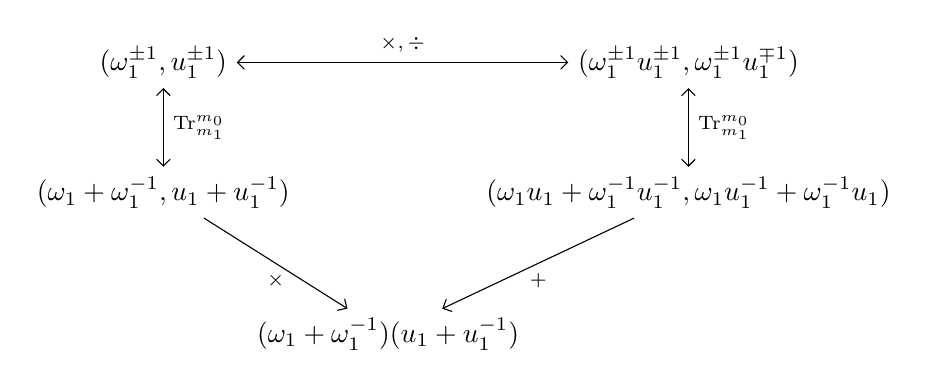
\begin{tikzpicture}
      \node (u) {$(\omega_1^{\pm 1}, u_1^{\pm 1})$};
      \node[below=of u] (to) {$(\omega_1+\omega_1^{-1}, u_1+u_1^{-1})$};
      \node[right=of to] (fake) {};
      \node[right=of fake] (rs) {$(\omega_1 u_1+\omega_1^{-1}u_1^{-1},\omega_1 u_1^{-1}+\omega_1^{-1} u_1)$};
      \node[above=of rs] (w) {$(\omega_1^{\pm 1}u_1^{\pm 1}, \omega_1^{\pm1} u_1^{\mp 1})$};
      \node[below=of fake, yshift=-1em] (eq) {$(\omega_1+\omega_1^{-1})(u_1+u_1^{-1})$};
      \path[<->,font=\scriptsize,>=angle 90]
      (u) edge node[above]{$\times, \div$} (w)
      (u) edge node[right]{$\tr[m_1]{m_0}{}$} (to)
      (w) edge node[right]{$\tr[m_1]{m_0}{}$} (rs);
      \path[->,font=\scriptsize,>=angle 90]
      (to) edge node[below]{$\times$} (eq)
      (rs) edge node[below]{$+$} (eq);
    \end{tikzpicture}
  \end{center}

  Not conclusive (yet?)
\end{frame}

\begin{frame}
  %Experimental evidence suggests the following formula stands.
  \begin{conjecture}
    If $K_{m_1}(a) \equiv 1 \pmod{3}$, then
    \begin{align*}
    \cthree{\Sigma_3} =
    & \quad \frac{2^{m_2+1} - K_{m_1}(a)}{3} \\
    & \qquad + 2 \tr{m_0}{a \omega_1^{2}} \frac{2^{m_2+1} - 1}{3} \\
    & \qquad - \mystery \addch{\tr{m_0}{a \omega_1^{2}}} 2^{m_2}
    \enspace .
    \end{align*}
  \end{conjecture}

  \vspace{2em}

  This does not give the full Walsh spectrum for all values of $a$, but proves that if $K_{m_1} = 4$ then $f_{a,b}$ is bent.
\end{frame}

\begin{frame}
  The conjecture was checked using a C/ASM program
  using \emph{AVX extensions} for the arithmetic of $\GF{m_0}^*$,
  \emph{PARI/GP} to compute the Kloosterman sums $K_{m_1}(a)$,
  and \emph{Pthreads} for parallelization.

  \vspace{2em}

  Complexity given by
  \begin{itemize}
  \item
    $3$ values of $\gamma \in \GF[4]{}^*$ to check,
  \item
    $\tilde{O}(2^{m_1})$ values of $a \in \GF{m_1}^*$ to check,
  \item
    $2^{m_1-1}$ values of $\omega_1 \in U_1 \backslash \set{1}$,
  \item
    $\tilde{O}(2^{m_1})$ operations in $\GF{m_0}$ for each $\omega_1$,
  \end{itemize}
  which amounts to \red{$\tilde{O}(2^{3 m_1})$}.

  \vspace{2em}

  It was done
  \begin{itemize}
  \item completely for $m_2 = 3, 5, 7, 9$,
  \item for $i$ up to about $2^{12}$ where $a = z^i$
    and $z$ is a primitive element of $\GF{m_1}$ for $m_2 = 11$.
  \end{itemize}
\end{frame}

\begin{frame}
  Similar techniques can be used when $n = 2^\nu m$ with $\nu \geq 2$.
  \begin{proposition}
    For $\nu > 1$, $a \in \GF{m_1}^*$ and $b \in \GF[4]{}^*$,
    and $\omega \in \GF{m_0}^*$,
    the Walsh transform of $f_{a,b}$ at $\omega \neq 0$ is
    \begin{align*}
      \WT{f_{a,b}}(\omega)
      & = 1 - \frac{2 \cdot 2^{\left(2^{\nu-1}-1\right)m_\nu} - 1}{3} \left(1 - K_{m_1}(a)\right) \\
      & \qquad - \frac{2 \cdot 2^{\left( 2^{\nu-1} - 1 \right) m_\nu} \left( 2^{m_\nu - 1} - 1 \right)}{3} \addch{f_a(\omega_1)} \\
      & \qquad + 2^{m_{\nu} + 1} \cthree{\sum_{\tr[m_{\nu-1}]{m_0}{u \omega} \neq 0, \tr[m_\nu]{m_0}{u \omega} = 0, b \mulch[m_0]{u_\nu} = 1} \addch{f_a(u_1)}} \enspace .
    \end{align*}

  \end{proposition}
  Unfortunately the unexplicit \cthree{last sum},
  corresponding to $\cthree{\Sigma_3}$ above is even harder to make explicit.
\end{frame}

\begin{frame}
  Many of the properties used here also apply when the \emph{cubic multiplicative character} is replaced by another multiplicative character.

  \vspace{2em}

  For example, there exist efficient characterizations involving
  Kloosterman sums and quintic sums for
  \[
  f_{a,b}(x) = \tr{n}{a x^{2^{n/2}-1}} + \tr{4}{b x^{(2^n - 1)/5}}
  \]
  when $n = 4m$ and $m$ is odd.

  Nothing is known when $m$ even.
\end{frame}

\begin{frame}[fragile=singleslide]
  \vfill
  \begin{center}
    \begin{minipage}{.7\linewidth}
\begin{verbatim}
   __________                            
  /          \                           
 ( QUESTIONS? )_  |\      _,,,--,,_      
  \__________/  \ /,`.-'`'   ._  \-;;,_  
                 |,4-  ) )_   .;.(  `'-'
                '---''(_/._)-'(_\_)     
\end{verbatim}
    \end{minipage}
  \end{center}
  \vfill
\end{frame}

\end{document}
